\documentclass[twoside]{book}

% Packages required by doxygen
\usepackage{calc}
\usepackage{doxygen}
\usepackage{graphicx}
\usepackage[utf8]{inputenc}
\usepackage{makeidx}
\usepackage{multicol}
\usepackage{multirow}
\usepackage{textcomp}
\usepackage[table]{xcolor}

% Font selection
\usepackage[T1]{fontenc}
\usepackage{mathptmx}
\usepackage[scaled=.90]{helvet}
\usepackage{courier}
\usepackage{amssymb}
\usepackage{sectsty}
\renewcommand{\familydefault}{\sfdefault}
\allsectionsfont{%
  \fontseries{bc}\selectfont%
  \color{darkgray}%
}
\renewcommand{\DoxyLabelFont}{%
  \fontseries{bc}\selectfont%
  \color{darkgray}%
}

% Page & text layout
\usepackage{geometry}
\geometry{%
  a4paper,%
  top=2.5cm,%
  bottom=2.5cm,%
  left=2.5cm,%
  right=2.5cm%
}
\tolerance=750
\hfuzz=15pt
\hbadness=750
\setlength{\emergencystretch}{15pt}
\setlength{\parindent}{0cm}
\setlength{\parskip}{0.2cm}
\makeatletter
\renewcommand{\paragraph}{%
  \@startsection{paragraph}{4}{0ex}{-1.0ex}{1.0ex}{%
    \normalfont\normalsize\bfseries\SS@parafont%
  }%
}
\renewcommand{\subparagraph}{%
  \@startsection{subparagraph}{5}{0ex}{-1.0ex}{1.0ex}{%
    \normalfont\normalsize\bfseries\SS@subparafont%
  }%
}
\makeatother

% Headers & footers
\usepackage{fancyhdr}
\pagestyle{fancyplain}
\fancyhead[LE]{\fancyplain{}{\bfseries\thepage}}
\fancyhead[CE]{\fancyplain{}{}}
\fancyhead[RE]{\fancyplain{}{\bfseries\leftmark}}
\fancyhead[LO]{\fancyplain{}{\bfseries\rightmark}}
\fancyhead[CO]{\fancyplain{}{}}
\fancyhead[RO]{\fancyplain{}{\bfseries\thepage}}
\fancyfoot[LE]{\fancyplain{}{}}
\fancyfoot[CE]{\fancyplain{}{}}
\fancyfoot[RE]{\fancyplain{}{\bfseries\scriptsize Generated on Thu Nov 14 2013 11\-:54\-:35 for My Project by Doxygen }}
\fancyfoot[LO]{\fancyplain{}{\bfseries\scriptsize Generated on Thu Nov 14 2013 11\-:54\-:35 for My Project by Doxygen }}
\fancyfoot[CO]{\fancyplain{}{}}
\fancyfoot[RO]{\fancyplain{}{}}
\renewcommand{\footrulewidth}{0.4pt}
\renewcommand{\chaptermark}[1]{%
  \markboth{#1}{}%
}
\renewcommand{\sectionmark}[1]{%
  \markright{\thesection\ #1}%
}

% Indices & bibliography
\usepackage{natbib}
\usepackage[titles]{tocloft}
\setcounter{tocdepth}{3}
\setcounter{secnumdepth}{5}
\makeindex

% Hyperlinks (required, but should be loaded last)
\usepackage{ifpdf}
\ifpdf
  \usepackage[pdftex,pagebackref=true]{hyperref}
\else
  \usepackage[ps2pdf,pagebackref=true]{hyperref}
\fi
\hypersetup{%
  colorlinks=true,%
  linkcolor=blue,%
  citecolor=blue,%
  unicode%
}

% Custom commands
\newcommand{\clearemptydoublepage}{%
  \newpage{\pagestyle{empty}\cleardoublepage}%
}


%===== C O N T E N T S =====

\begin{document}

% Titlepage & ToC
\hypersetup{pageanchor=false}
\pagenumbering{roman}
\begin{titlepage}
\vspace*{7cm}
\begin{center}%
{\Large My Project }\\
\vspace*{1cm}
{\large Generated by Doxygen 1.8.5}\\
\vspace*{0.5cm}
{\small Thu Nov 14 2013 11:54:35}\\
\end{center}
\end{titlepage}
\clearemptydoublepage
\tableofcontents
\clearemptydoublepage
\pagenumbering{arabic}
\hypersetup{pageanchor=true}

%--- Begin generated contents ---
\chapter{Hierarchical Index}
\section{Class Hierarchy}
This inheritance list is sorted roughly, but not completely, alphabetically\-:\begin{DoxyCompactList}
\item Q\-Object\begin{DoxyCompactList}
\item \contentsline{section}{Penguin\-Server\-:\-:Connected\-Client}{\pageref{classPenguinServer_1_1ConnectedClient}}{}
\item \contentsline{section}{Penguin\-Server\-:\-:Shared\-List}{\pageref{classPenguinServer_1_1SharedList}}{}
\end{DoxyCompactList}
\item Q\-Tcp\-Server\begin{DoxyCompactList}
\item \contentsline{section}{Penguin\-Server\-:\-:Server\-Listener}{\pageref{classPenguinServer_1_1ServerListener}}{}
\end{DoxyCompactList}
\item Q\-Thread\begin{DoxyCompactList}
\item \contentsline{section}{Penguin\-Server\-:\-:Clients\-Manager}{\pageref{classPenguinServer_1_1ClientsManager}}{}
\item \contentsline{section}{Penguin\-Server\-:\-:Controler}{\pageref{classPenguinServer_1_1Controler}}{}
\item \contentsline{section}{Penguin\-Server\-:\-:Server\-Thread}{\pageref{classPenguinServer_1_1ServerThread}}{}
\end{DoxyCompactList}
\end{DoxyCompactList}

\chapter{Class Index}
\section{Class List}
Here are the classes, structs, unions and interfaces with brief descriptions\-:\begin{DoxyCompactList}
\item\contentsline{section}{\hyperlink{classPenguinServer_1_1ClientsManager}{Penguin\-Server\-::\-Clients\-Manager} \\*The \hyperlink{classPenguinServer_1_1ClientsManager}{Clients\-Manager} class This class represents manager of all clients. Curently this manager is responsible for resending the Clients list, but for the future will be used to manage all other issues checking state of communication and other }{\pageref{classPenguinServer_1_1ClientsManager}}{}
\item\contentsline{section}{\hyperlink{classPenguinServer_1_1ConnectedClient}{Penguin\-Server\-::\-Connected\-Client} \\*The \hyperlink{classPenguinServer_1_1ConnectedClient}{Connected\-Client} class Class represents data of client in system. Is connected to \hyperlink{classPenguinServer_1_1ServerThread}{Server\-Thread} which is operating all incomming and outcomming data }{\pageref{classPenguinServer_1_1ConnectedClient}}{}
\item\contentsline{section}{\hyperlink{classPenguinServer_1_1Controler}{Penguin\-Server\-::\-Controler} }{\pageref{classPenguinServer_1_1Controler}}{}
\item\contentsline{section}{\hyperlink{classPenguinServer_1_1ServerListener}{Penguin\-Server\-::\-Server\-Listener} \\*The \hyperlink{classPenguinServer_1_1ServerListener}{Server\-Listener} class Class represents a Tcp Listenere which manages all incomming calls }{\pageref{classPenguinServer_1_1ServerListener}}{}
\item\contentsline{section}{\hyperlink{classPenguinServer_1_1ServerThread}{Penguin\-Server\-::\-Server\-Thread} }{\pageref{classPenguinServer_1_1ServerThread}}{}
\item\contentsline{section}{\hyperlink{classPenguinServer_1_1SharedList}{Penguin\-Server\-::\-Shared\-List} \\*The \hyperlink{classPenguinServer_1_1SharedList}{Shared\-List} class }{\pageref{classPenguinServer_1_1SharedList}}{}
\end{DoxyCompactList}

\chapter{Class Documentation}
\hypertarget{classPenguinServer_1_1ClientsManager}{\section{Penguin\-Server\-:\-:Clients\-Manager Class Reference}
\label{classPenguinServer_1_1ClientsManager}\index{Penguin\-Server\-::\-Clients\-Manager@{Penguin\-Server\-::\-Clients\-Manager}}
}


The \hyperlink{classPenguinServer_1_1ClientsManager}{Clients\-Manager} class This class represents manager of all clients. Curently this manager is responsible for resending the Clients list, but for the future will be used to manage all other issues checking state of communication and other.  




{\ttfamily \#include $<$clientsmanager.\-h$>$}

Inheritance diagram for Penguin\-Server\-:\-:Clients\-Manager\-:\begin{figure}[H]
\begin{center}
\leavevmode
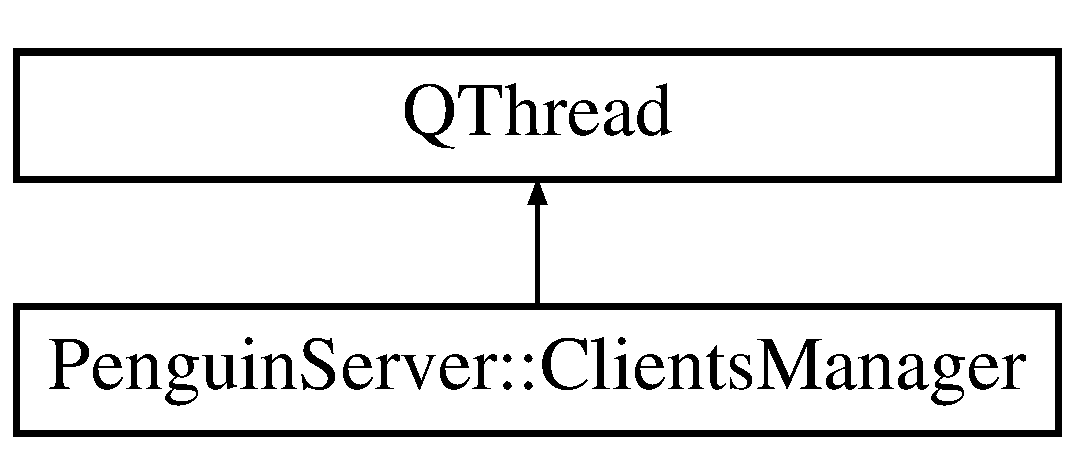
\includegraphics[height=2.000000cm]{classPenguinServer_1_1ClientsManager}
\end{center}
\end{figure}
\subsection*{Public Member Functions}
\begin{DoxyCompactItemize}
\item 
\hyperlink{classPenguinServer_1_1ClientsManager_a69c4459061b69d57b8df6b246afe5baa}{Clients\-Manager} (\hyperlink{classPenguinServer_1_1SharedList}{Shared\-List} $\ast$l, Q\-Object $\ast$parent=0)
\begin{DoxyCompactList}\small\item\em \hyperlink{classPenguinServer_1_1ClientsManager}{Clients\-Manager} constructor. \end{DoxyCompactList}\item 
\hypertarget{classPenguinServer_1_1ClientsManager_aae3e1462ada1fdac7b06dd4367f2ddd1}{void \hyperlink{classPenguinServer_1_1ClientsManager_aae3e1462ada1fdac7b06dd4367f2ddd1}{run} ()}\label{classPenguinServer_1_1ClientsManager_aae3e1462ada1fdac7b06dd4367f2ddd1}

\begin{DoxyCompactList}\small\item\em run abstract metod inhered from Q\-Thread runs the loop which emits the data send signal. \end{DoxyCompactList}\item 
void \hyperlink{classPenguinServer_1_1ClientsManager_ad2450664a05868d6581534a3994acfe2}{set\-List} (\hyperlink{classPenguinServer_1_1SharedList}{Shared\-List} $\ast$l)
\begin{DoxyCompactList}\small\item\em set\-List \end{DoxyCompactList}\end{DoxyCompactItemize}


\subsection{Detailed Description}
The \hyperlink{classPenguinServer_1_1ClientsManager}{Clients\-Manager} class This class represents manager of all clients. Curently this manager is responsible for resending the Clients list, but for the future will be used to manage all other issues checking state of communication and other. 

\subsection{Constructor \& Destructor Documentation}
\hypertarget{classPenguinServer_1_1ClientsManager_a69c4459061b69d57b8df6b246afe5baa}{\index{Penguin\-Server\-::\-Clients\-Manager@{Penguin\-Server\-::\-Clients\-Manager}!Clients\-Manager@{Clients\-Manager}}
\index{Clients\-Manager@{Clients\-Manager}!PenguinServer::ClientsManager@{Penguin\-Server\-::\-Clients\-Manager}}
\subsubsection[{Clients\-Manager}]{\setlength{\rightskip}{0pt plus 5cm}Penguin\-Server\-::\-Clients\-Manager\-::\-Clients\-Manager (
\begin{DoxyParamCaption}
\item[{{\bf Shared\-List} $\ast$}]{l, }
\item[{Q\-Object $\ast$}]{parent = {\ttfamily 0}}
\end{DoxyParamCaption}
)\hspace{0.3cm}{\ttfamily [inline]}}}\label{classPenguinServer_1_1ClientsManager_a69c4459061b69d57b8df6b246afe5baa}


\hyperlink{classPenguinServer_1_1ClientsManager}{Clients\-Manager} constructor. 


\begin{DoxyParams}{Parameters}
{\em l} & The shared list to work with \\
\hline
{\em parent} & -\/ The parent of object \\
\hline
\end{DoxyParams}


\subsection{Member Function Documentation}
\hypertarget{classPenguinServer_1_1ClientsManager_ad2450664a05868d6581534a3994acfe2}{\index{Penguin\-Server\-::\-Clients\-Manager@{Penguin\-Server\-::\-Clients\-Manager}!set\-List@{set\-List}}
\index{set\-List@{set\-List}!PenguinServer::ClientsManager@{Penguin\-Server\-::\-Clients\-Manager}}
\subsubsection[{set\-List}]{\setlength{\rightskip}{0pt plus 5cm}void Penguin\-Server\-::\-Clients\-Manager\-::set\-List (
\begin{DoxyParamCaption}
\item[{{\bf Shared\-List} $\ast$}]{l}
\end{DoxyParamCaption}
)}}\label{classPenguinServer_1_1ClientsManager_ad2450664a05868d6581534a3994acfe2}


set\-List 


\begin{DoxyParams}{Parameters}
{\em l} & \\
\hline
\end{DoxyParams}


The documentation for this class was generated from the following files\-:\begin{DoxyCompactItemize}
\item 
clientsmanager.\-h\item 
clientsmanager.\-cpp\end{DoxyCompactItemize}

\hypertarget{classPenguinServer_1_1ConnectedClient}{\section{Penguin\-Server\-:\-:Connected\-Client Class Reference}
\label{classPenguinServer_1_1ConnectedClient}\index{Penguin\-Server\-::\-Connected\-Client@{Penguin\-Server\-::\-Connected\-Client}}
}


The \hyperlink{classPenguinServer_1_1ConnectedClient}{Connected\-Client} class Class represents data of client in system. Is connected to \hyperlink{classPenguinServer_1_1ServerThread}{Server\-Thread} which is operating all incomming and outcomming data.  




{\ttfamily \#include $<$connectedclient.\-h$>$}

Inheritance diagram for Penguin\-Server\-:\-:Connected\-Client\-:\begin{figure}[H]
\begin{center}
\leavevmode
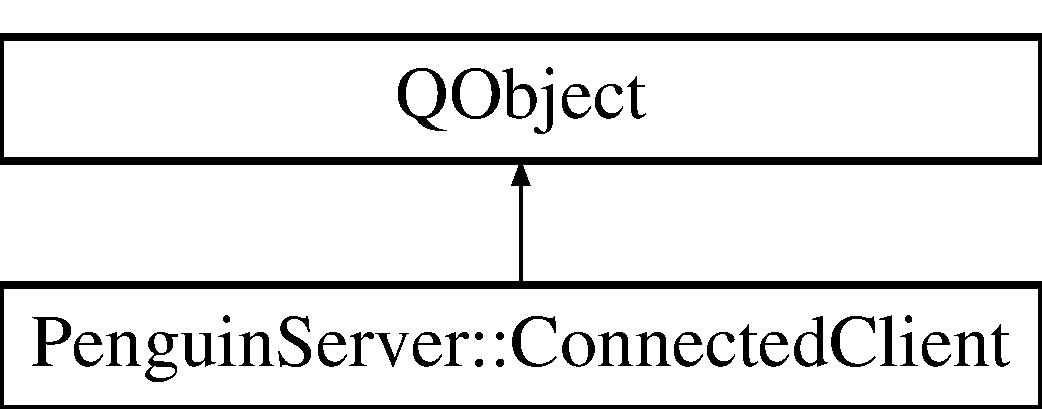
\includegraphics[height=2.000000cm]{classPenguinServer_1_1ConnectedClient}
\end{center}
\end{figure}
\subsection*{Signals}
\begin{DoxyCompactItemize}
\item 
void \hyperlink{classPenguinServer_1_1ConnectedClient_a9040ba0b51fb32e9bf8736aaa6e59b4d}{send\-Updated\-List} (Q\-List$<$ Q\-String $>$ s)
\begin{DoxyCompactList}\small\item\em send\-Updated\-List \end{DoxyCompactList}\item 
\hypertarget{classPenguinServer_1_1ConnectedClient_af4082cf1b1b69c21fbdec855d951f910}{void \hyperlink{classPenguinServer_1_1ConnectedClient_af4082cf1b1b69c21fbdec855d951f910}{request\-Connection} (\hyperlink{classPenguinServer_1_1ConnectedClient}{Connected\-Client} $\ast$)}\label{classPenguinServer_1_1ConnectedClient_af4082cf1b1b69c21fbdec855d951f910}

\begin{DoxyCompactList}\small\item\em request\-Connection \end{DoxyCompactList}\item 
\hypertarget{classPenguinServer_1_1ConnectedClient_a10f32c661b8146c904b111aa347f37cb}{void \hyperlink{classPenguinServer_1_1ConnectedClient_a10f32c661b8146c904b111aa347f37cb}{deny\-Connection} (\hyperlink{classPenguinServer_1_1ConnectedClient}{Connected\-Client} $\ast$)}\label{classPenguinServer_1_1ConnectedClient_a10f32c661b8146c904b111aa347f37cb}

\begin{DoxyCompactList}\small\item\em deny\-Connection \end{DoxyCompactList}\item 
\hypertarget{classPenguinServer_1_1ConnectedClient_acec0bf4652332010b498ca5cfcc29627}{void \hyperlink{classPenguinServer_1_1ConnectedClient_acec0bf4652332010b498ca5cfcc29627}{allow\-Connection} (\hyperlink{classPenguinServer_1_1ConnectedClient}{Connected\-Client} $\ast$)}\label{classPenguinServer_1_1ConnectedClient_acec0bf4652332010b498ca5cfcc29627}

\begin{DoxyCompactList}\small\item\em allow\-Connection \end{DoxyCompactList}\end{DoxyCompactItemize}
\subsection*{Public Member Functions}
\begin{DoxyCompactItemize}
\item 
\hyperlink{classPenguinServer_1_1ConnectedClient_a2167c805df33e4a18d40b7078f3023ae}{Connected\-Client} (Q\-Host\-Address ip\-Addr, Q\-String name, qint16 port, \hyperlink{classPenguinServer_1_1ServerThread}{Server\-Thread} $\ast$parent=0)
\begin{DoxyCompactList}\small\item\em \hyperlink{classPenguinServer_1_1ConnectedClient}{Connected\-Client} constructor. \end{DoxyCompactList}\item 
Q\-String \hyperlink{classPenguinServer_1_1ConnectedClient_afd5c19ed689f899e464eed48a6e80038}{get\-Name} ()
\begin{DoxyCompactList}\small\item\em get\-Name \end{DoxyCompactList}\item 
qint16 \hyperlink{classPenguinServer_1_1ConnectedClient_ad263530695c1806cbbb0070fce6552d9}{get\-Port} ()
\begin{DoxyCompactList}\small\item\em get\-Port \end{DoxyCompactList}\item 
Q\-Host\-Address \hyperlink{classPenguinServer_1_1ConnectedClient_aecc94c3bcb3bee9740d10173eb73160c}{get\-Ip\-Addr} ()
\begin{DoxyCompactList}\small\item\em get\-Ip\-Addr \end{DoxyCompactList}\item 
void \hyperlink{classPenguinServer_1_1ConnectedClient_a61c876737001fd3dfb06f6cd69d255d9}{call\-Request} (int req\-Id, \hyperlink{classPenguinServer_1_1ConnectedClient}{Connected\-Client} $\ast$cli)
\begin{DoxyCompactList}\small\item\em call\-Request Calls request -\/ emits signal, to Thread to send data from another client \end{DoxyCompactList}\item 
void \hyperlink{classPenguinServer_1_1ConnectedClient_ae14d3b2ae3096c527ba387c8b204af40}{send\-List} (Q\-List$<$ Q\-String $>$ list)
\begin{DoxyCompactList}\small\item\em send\-List Sends list of clients to this client -\/ emits signal \end{DoxyCompactList}\item 
void \hyperlink{classPenguinServer_1_1ConnectedClient_a89d4ee61c9736341d640b2d7edafae3b}{init} (\hyperlink{classPenguinServer_1_1ServerThread}{Server\-Thread} $\ast$parent)
\begin{DoxyCompactList}\small\item\em init Initializes the conectivity to parent thread, connects this signalst to parent-\/$>$slots \end{DoxyCompactList}\end{DoxyCompactItemize}


\subsection{Detailed Description}
The \hyperlink{classPenguinServer_1_1ConnectedClient}{Connected\-Client} class Class represents data of client in system. Is connected to \hyperlink{classPenguinServer_1_1ServerThread}{Server\-Thread} which is operating all incomming and outcomming data. 

\subsection{Constructor \& Destructor Documentation}
\hypertarget{classPenguinServer_1_1ConnectedClient_a2167c805df33e4a18d40b7078f3023ae}{\index{Penguin\-Server\-::\-Connected\-Client@{Penguin\-Server\-::\-Connected\-Client}!Connected\-Client@{Connected\-Client}}
\index{Connected\-Client@{Connected\-Client}!PenguinServer::ConnectedClient@{Penguin\-Server\-::\-Connected\-Client}}
\subsubsection[{Connected\-Client}]{\setlength{\rightskip}{0pt plus 5cm}Penguin\-Server\-::\-Connected\-Client\-::\-Connected\-Client (
\begin{DoxyParamCaption}
\item[{Q\-Host\-Address}]{ip\-Addr, }
\item[{Q\-String}]{name, }
\item[{qint16}]{port, }
\item[{{\bf Server\-Thread} $\ast$}]{parent = {\ttfamily 0}}
\end{DoxyParamCaption}
)}}\label{classPenguinServer_1_1ConnectedClient_a2167c805df33e4a18d40b7078f3023ae}


\hyperlink{classPenguinServer_1_1ConnectedClient}{Connected\-Client} constructor. 


\begin{DoxyParams}{Parameters}
{\em ip\-Addr} & Address of the client \\
\hline
{\em name} & name of the client \\
\hline
{\em port} & port which is used to communication \\
\hline
{\em parent} & Q\-Object \\
\hline
\end{DoxyParams}


\subsection{Member Function Documentation}
\hypertarget{classPenguinServer_1_1ConnectedClient_a61c876737001fd3dfb06f6cd69d255d9}{\index{Penguin\-Server\-::\-Connected\-Client@{Penguin\-Server\-::\-Connected\-Client}!call\-Request@{call\-Request}}
\index{call\-Request@{call\-Request}!PenguinServer::ConnectedClient@{Penguin\-Server\-::\-Connected\-Client}}
\subsubsection[{call\-Request}]{\setlength{\rightskip}{0pt plus 5cm}void Penguin\-Server\-::\-Connected\-Client\-::call\-Request (
\begin{DoxyParamCaption}
\item[{int}]{req\-Id, }
\item[{{\bf Connected\-Client} $\ast$}]{cli}
\end{DoxyParamCaption}
)}}\label{classPenguinServer_1_1ConnectedClient_a61c876737001fd3dfb06f6cd69d255d9}


call\-Request Calls request -\/ emits signal, to Thread to send data from another client 


\begin{DoxyParams}{Parameters}
{\em req\-Id} & I\-D of request more in ../messageenvelop.h \\
\hline
{\em cli} & client whose data mus be sent \\
\hline
\end{DoxyParams}
\hypertarget{classPenguinServer_1_1ConnectedClient_aecc94c3bcb3bee9740d10173eb73160c}{\index{Penguin\-Server\-::\-Connected\-Client@{Penguin\-Server\-::\-Connected\-Client}!get\-Ip\-Addr@{get\-Ip\-Addr}}
\index{get\-Ip\-Addr@{get\-Ip\-Addr}!PenguinServer::ConnectedClient@{Penguin\-Server\-::\-Connected\-Client}}
\subsubsection[{get\-Ip\-Addr}]{\setlength{\rightskip}{0pt plus 5cm}Q\-Host\-Address Penguin\-Server\-::\-Connected\-Client\-::get\-Ip\-Addr (
\begin{DoxyParamCaption}
{}
\end{DoxyParamCaption}
)}}\label{classPenguinServer_1_1ConnectedClient_aecc94c3bcb3bee9740d10173eb73160c}


get\-Ip\-Addr 

\begin{DoxyReturn}{Returns}
ip address 
\end{DoxyReturn}
\hypertarget{classPenguinServer_1_1ConnectedClient_afd5c19ed689f899e464eed48a6e80038}{\index{Penguin\-Server\-::\-Connected\-Client@{Penguin\-Server\-::\-Connected\-Client}!get\-Name@{get\-Name}}
\index{get\-Name@{get\-Name}!PenguinServer::ConnectedClient@{Penguin\-Server\-::\-Connected\-Client}}
\subsubsection[{get\-Name}]{\setlength{\rightskip}{0pt plus 5cm}Q\-String Penguin\-Server\-::\-Connected\-Client\-::get\-Name (
\begin{DoxyParamCaption}
{}
\end{DoxyParamCaption}
)}}\label{classPenguinServer_1_1ConnectedClient_afd5c19ed689f899e464eed48a6e80038}


get\-Name 

\begin{DoxyReturn}{Returns}
name 
\end{DoxyReturn}
\hypertarget{classPenguinServer_1_1ConnectedClient_ad263530695c1806cbbb0070fce6552d9}{\index{Penguin\-Server\-::\-Connected\-Client@{Penguin\-Server\-::\-Connected\-Client}!get\-Port@{get\-Port}}
\index{get\-Port@{get\-Port}!PenguinServer::ConnectedClient@{Penguin\-Server\-::\-Connected\-Client}}
\subsubsection[{get\-Port}]{\setlength{\rightskip}{0pt plus 5cm}qint16 Penguin\-Server\-::\-Connected\-Client\-::get\-Port (
\begin{DoxyParamCaption}
{}
\end{DoxyParamCaption}
)}}\label{classPenguinServer_1_1ConnectedClient_ad263530695c1806cbbb0070fce6552d9}


get\-Port 

\begin{DoxyReturn}{Returns}
port number 
\end{DoxyReturn}
\hypertarget{classPenguinServer_1_1ConnectedClient_a89d4ee61c9736341d640b2d7edafae3b}{\index{Penguin\-Server\-::\-Connected\-Client@{Penguin\-Server\-::\-Connected\-Client}!init@{init}}
\index{init@{init}!PenguinServer::ConnectedClient@{Penguin\-Server\-::\-Connected\-Client}}
\subsubsection[{init}]{\setlength{\rightskip}{0pt plus 5cm}void Penguin\-Server\-::\-Connected\-Client\-::init (
\begin{DoxyParamCaption}
\item[{{\bf Server\-Thread} $\ast$}]{parent}
\end{DoxyParamCaption}
)}}\label{classPenguinServer_1_1ConnectedClient_a89d4ee61c9736341d640b2d7edafae3b}


init Initializes the conectivity to parent thread, connects this signalst to parent-\/$>$slots 


\begin{DoxyParams}{Parameters}
{\em parent} & \\
\hline
\end{DoxyParams}
\hypertarget{classPenguinServer_1_1ConnectedClient_ae14d3b2ae3096c527ba387c8b204af40}{\index{Penguin\-Server\-::\-Connected\-Client@{Penguin\-Server\-::\-Connected\-Client}!send\-List@{send\-List}}
\index{send\-List@{send\-List}!PenguinServer::ConnectedClient@{Penguin\-Server\-::\-Connected\-Client}}
\subsubsection[{send\-List}]{\setlength{\rightskip}{0pt plus 5cm}void Penguin\-Server\-::\-Connected\-Client\-::send\-List (
\begin{DoxyParamCaption}
\item[{Q\-List$<$ Q\-String $>$}]{list}
\end{DoxyParamCaption}
)}}\label{classPenguinServer_1_1ConnectedClient_ae14d3b2ae3096c527ba387c8b204af40}


send\-List Sends list of clients to this client -\/ emits signal 


\begin{DoxyParams}{Parameters}
{\em list} & data to be sent \\
\hline
\end{DoxyParams}
\hypertarget{classPenguinServer_1_1ConnectedClient_a9040ba0b51fb32e9bf8736aaa6e59b4d}{\index{Penguin\-Server\-::\-Connected\-Client@{Penguin\-Server\-::\-Connected\-Client}!send\-Updated\-List@{send\-Updated\-List}}
\index{send\-Updated\-List@{send\-Updated\-List}!PenguinServer::ConnectedClient@{Penguin\-Server\-::\-Connected\-Client}}
\subsubsection[{send\-Updated\-List}]{\setlength{\rightskip}{0pt plus 5cm}void Penguin\-Server\-::\-Connected\-Client\-::send\-Updated\-List (
\begin{DoxyParamCaption}
\item[{Q\-List$<$ Q\-String $>$}]{s}
\end{DoxyParamCaption}
)\hspace{0.3cm}{\ttfamily [signal]}}}\label{classPenguinServer_1_1ConnectedClient_a9040ba0b51fb32e9bf8736aaa6e59b4d}


send\-Updated\-List 


\begin{DoxyParams}{Parameters}
{\em s} & \\
\hline
\end{DoxyParams}


The documentation for this class was generated from the following files\-:\begin{DoxyCompactItemize}
\item 
connectedclient.\-h\item 
connectedclient.\-cpp\end{DoxyCompactItemize}

\hypertarget{classPenguinServer_1_1Controler}{\section{Penguin\-Server\-:\-:Controler Class Reference}
\label{classPenguinServer_1_1Controler}\index{Penguin\-Server\-::\-Controler@{Penguin\-Server\-::\-Controler}}
}
Inheritance diagram for Penguin\-Server\-:\-:Controler\-:\begin{figure}[H]
\begin{center}
\leavevmode
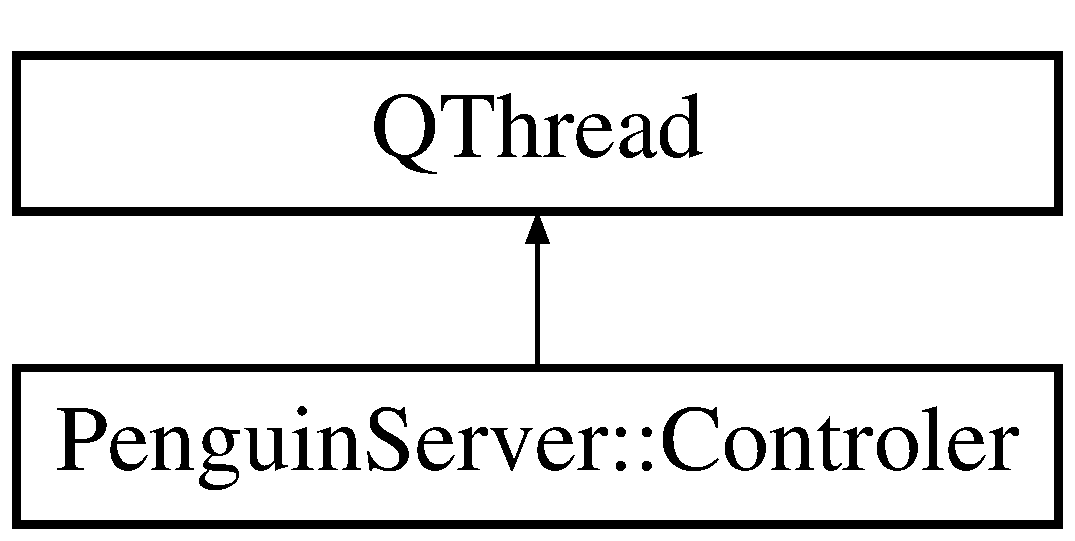
\includegraphics[height=2.000000cm]{classPenguinServer_1_1Controler}
\end{center}
\end{figure}
\subsection*{Signals}
\begin{DoxyCompactItemize}
\item 
\hypertarget{classPenguinServer_1_1Controler_a9d688185332790c948fc25bdf1da96a6}{void {\bfseries finish} ()}\label{classPenguinServer_1_1Controler_a9d688185332790c948fc25bdf1da96a6}

\end{DoxyCompactItemize}
\subsection*{Public Member Functions}
\begin{DoxyCompactItemize}
\item 
\hypertarget{classPenguinServer_1_1Controler_a553892788a017f926fc4669ff5062612}{{\bfseries Controler} (Q\-Object $\ast$parent=0)}\label{classPenguinServer_1_1Controler_a553892788a017f926fc4669ff5062612}

\item 
\hypertarget{classPenguinServer_1_1Controler_a25d46a60f87ec8a30ba7a447bc52f12a}{virtual void {\bfseries run} ()}\label{classPenguinServer_1_1Controler_a25d46a60f87ec8a30ba7a447bc52f12a}

\end{DoxyCompactItemize}


The documentation for this class was generated from the following files\-:\begin{DoxyCompactItemize}
\item 
serverlistener.\-h\item 
main.\-cpp\end{DoxyCompactItemize}

\hypertarget{classPenguinServer_1_1ServerListener}{\section{Penguin\-Server\-:\-:Server\-Listener Class Reference}
\label{classPenguinServer_1_1ServerListener}\index{Penguin\-Server\-::\-Server\-Listener@{Penguin\-Server\-::\-Server\-Listener}}
}


The \hyperlink{classPenguinServer_1_1ServerListener}{Server\-Listener} class Class represents a Tcp Listenere which manages all incomming calls.  




{\ttfamily \#include $<$serverlistener.\-h$>$}

Inheritance diagram for Penguin\-Server\-:\-:Server\-Listener\-:\begin{figure}[H]
\begin{center}
\leavevmode
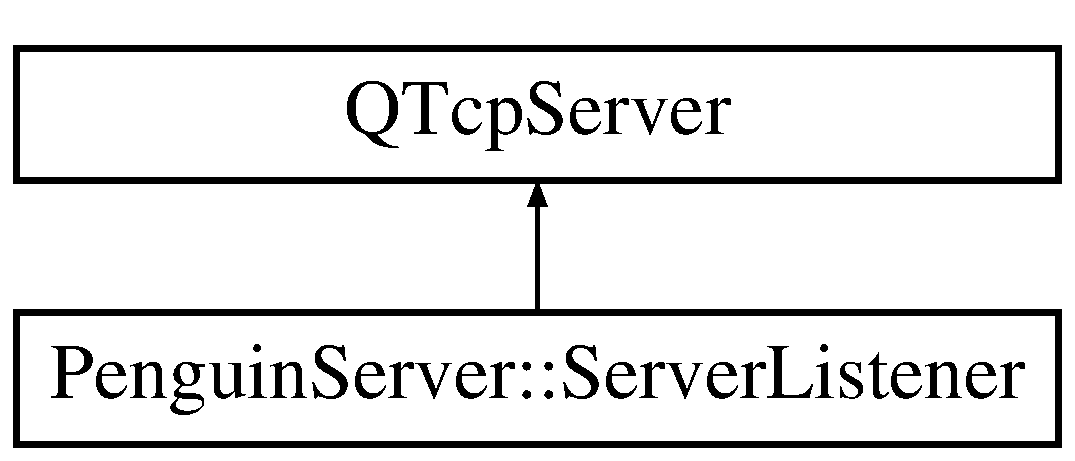
\includegraphics[height=2.000000cm]{classPenguinServer_1_1ServerListener}
\end{center}
\end{figure}
\subsection*{Public Member Functions}
\begin{DoxyCompactItemize}
\item 
\hyperlink{classPenguinServer_1_1ServerListener_a50619f2b21ddf6a4b6d534f984be2323}{Server\-Listener} (Q\-Object $\ast$parent=0)
\begin{DoxyCompactList}\small\item\em \hyperlink{classPenguinServer_1_1ServerListener}{Server\-Listener}. \end{DoxyCompactList}\item 
\hypertarget{classPenguinServer_1_1ServerListener_a070db48538948282b6cc6a0a2eb7682e}{void {\bfseries start} ()}\label{classPenguinServer_1_1ServerListener_a070db48538948282b6cc6a0a2eb7682e}

\end{DoxyCompactItemize}
\subsection*{Protected Member Functions}
\begin{DoxyCompactItemize}
\item 
\hypertarget{classPenguinServer_1_1ServerListener_acf6d1127a2f9e121b24fae142a4070f5}{void {\bfseries incoming\-Connection} (qintptr handle)}\label{classPenguinServer_1_1ServerListener_acf6d1127a2f9e121b24fae142a4070f5}

\end{DoxyCompactItemize}


\subsection{Detailed Description}
The \hyperlink{classPenguinServer_1_1ServerListener}{Server\-Listener} class Class represents a Tcp Listenere which manages all incomming calls. 

\subsection{Constructor \& Destructor Documentation}
\hypertarget{classPenguinServer_1_1ServerListener_a50619f2b21ddf6a4b6d534f984be2323}{\index{Penguin\-Server\-::\-Server\-Listener@{Penguin\-Server\-::\-Server\-Listener}!Server\-Listener@{Server\-Listener}}
\index{Server\-Listener@{Server\-Listener}!PenguinServer::ServerListener@{Penguin\-Server\-::\-Server\-Listener}}
\subsubsection[{Server\-Listener}]{\setlength{\rightskip}{0pt plus 5cm}Penguin\-Server\-::\-Server\-Listener\-::\-Server\-Listener (
\begin{DoxyParamCaption}
\item[{Q\-Object $\ast$}]{parent = {\ttfamily 0}}
\end{DoxyParamCaption}
)\hspace{0.3cm}{\ttfamily [explicit]}}}\label{classPenguinServer_1_1ServerListener_a50619f2b21ddf6a4b6d534f984be2323}


\hyperlink{classPenguinServer_1_1ServerListener}{Server\-Listener}. 


\begin{DoxyParams}{Parameters}
{\em parent} & \\
\hline
\end{DoxyParams}


The documentation for this class was generated from the following files\-:\begin{DoxyCompactItemize}
\item 
serverlistener.\-h\item 
serverlistener.\-cpp\end{DoxyCompactItemize}

\hypertarget{classPenguinServer_1_1ServerThread}{\section{Penguin\-Server\-:\-:Server\-Thread Class Reference}
\label{classPenguinServer_1_1ServerThread}\index{Penguin\-Server\-::\-Server\-Thread@{Penguin\-Server\-::\-Server\-Thread}}
}
Inheritance diagram for Penguin\-Server\-:\-:Server\-Thread\-:\begin{figure}[H]
\begin{center}
\leavevmode
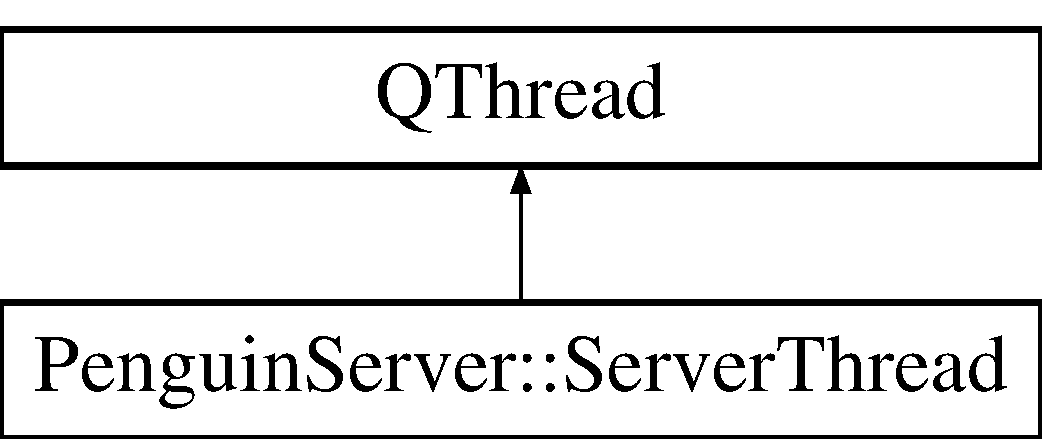
\includegraphics[height=2.000000cm]{classPenguinServer_1_1ServerThread}
\end{center}
\end{figure}
\subsection*{Public Slots}
\begin{DoxyCompactItemize}
\item 
void \hyperlink{classPenguinServer_1_1ServerThread_a5505bcb3b0bb4483859c59c38636585c}{distribute\-Clients} (Q\-List$<$ Q\-String $>$ list)
\begin{DoxyCompactList}\small\item\em distribute\-Clients \end{DoxyCompactList}\item 
\hypertarget{classPenguinServer_1_1ServerThread_a7f1c00042c85effe5d3e60b102d154ec}{void \hyperlink{classPenguinServer_1_1ServerThread_a7f1c00042c85effe5d3e60b102d154ec}{ask\-New\-Connection} (\hyperlink{classPenguinServer_1_1ConnectedClient}{Connected\-Client} $\ast$)}\label{classPenguinServer_1_1ServerThread_a7f1c00042c85effe5d3e60b102d154ec}

\begin{DoxyCompactList}\small\item\em ask\-New\-Connection \end{DoxyCompactList}\item 
\hypertarget{classPenguinServer_1_1ServerThread_ad6c087d78aa5dd7ed110be45a0c7b446}{void \hyperlink{classPenguinServer_1_1ServerThread_ad6c087d78aa5dd7ed110be45a0c7b446}{connection\-On\-Success} (\hyperlink{classPenguinServer_1_1ConnectedClient}{Connected\-Client} $\ast$)}\label{classPenguinServer_1_1ServerThread_ad6c087d78aa5dd7ed110be45a0c7b446}

\begin{DoxyCompactList}\small\item\em connection\-On\-Success \end{DoxyCompactList}\item 
\hypertarget{classPenguinServer_1_1ServerThread_afe59ece0b17da4749e342ec14c7891c4}{void \hyperlink{classPenguinServer_1_1ServerThread_afe59ece0b17da4749e342ec14c7891c4}{connection\-Denied} (\hyperlink{classPenguinServer_1_1ConnectedClient}{Connected\-Client} $\ast$)}\label{classPenguinServer_1_1ServerThread_afe59ece0b17da4749e342ec14c7891c4}

\begin{DoxyCompactList}\small\item\em connection\-Denied \end{DoxyCompactList}\item 
\hypertarget{classPenguinServer_1_1ServerThread_aab8eccde8e140e9ba81c7b566208f8de}{void \hyperlink{classPenguinServer_1_1ServerThread_aab8eccde8e140e9ba81c7b566208f8de}{ready\-Read} ()}\label{classPenguinServer_1_1ServerThread_aab8eccde8e140e9ba81c7b566208f8de}

\begin{DoxyCompactList}\small\item\em ready\-Read \end{DoxyCompactList}\item 
\hypertarget{classPenguinServer_1_1ServerThread_ab8cf109db69f19384009aa826a35a0d8}{void \hyperlink{classPenguinServer_1_1ServerThread_ab8cf109db69f19384009aa826a35a0d8}{disconnected} ()}\label{classPenguinServer_1_1ServerThread_ab8cf109db69f19384009aa826a35a0d8}

\begin{DoxyCompactList}\small\item\em disconnected \end{DoxyCompactList}\end{DoxyCompactItemize}
\subsection*{Signals}
\begin{DoxyCompactItemize}
\item 
\hypertarget{classPenguinServer_1_1ServerThread_a58b8482b6549f66c8f505dbc220579c5}{void {\bfseries error} (Q\-Tcp\-Socket\-::\-Socket\-Error err)}\label{classPenguinServer_1_1ServerThread_a58b8482b6549f66c8f505dbc220579c5}

\item 
\hypertarget{classPenguinServer_1_1ServerThread_ab0224bcf7968eadb0de910743935bec0}{void {\bfseries error} ()}\label{classPenguinServer_1_1ServerThread_ab0224bcf7968eadb0de910743935bec0}

\end{DoxyCompactItemize}
\subsection*{Public Member Functions}
\begin{DoxyCompactItemize}
\item 
\hyperlink{classPenguinServer_1_1ServerThread_a6cab741c43bc6d0794b019115d7a1b51}{Server\-Thread} (qintptr socket\-Descriptor, \hyperlink{classPenguinServer_1_1SharedList}{Shared\-List} $\ast$list, Q\-Object $\ast$parent=0)
\begin{DoxyCompactList}\small\item\em \hyperlink{classPenguinServer_1_1ServerThread}{Server\-Thread}. \end{DoxyCompactList}\item 
\hypertarget{classPenguinServer_1_1ServerThread_aaa5ec990ecfab27ee20f24e4c4992c6e}{void {\bfseries run} ()}\label{classPenguinServer_1_1ServerThread_aaa5ec990ecfab27ee20f24e4c4992c6e}

\end{DoxyCompactItemize}


\subsection{Constructor \& Destructor Documentation}
\hypertarget{classPenguinServer_1_1ServerThread_a6cab741c43bc6d0794b019115d7a1b51}{\index{Penguin\-Server\-::\-Server\-Thread@{Penguin\-Server\-::\-Server\-Thread}!Server\-Thread@{Server\-Thread}}
\index{Server\-Thread@{Server\-Thread}!PenguinServer::ServerThread@{Penguin\-Server\-::\-Server\-Thread}}
\subsubsection[{Server\-Thread}]{\setlength{\rightskip}{0pt plus 5cm}Penguin\-Server\-::\-Server\-Thread\-::\-Server\-Thread (
\begin{DoxyParamCaption}
\item[{qintptr}]{socket\-Descriptor, }
\item[{{\bf Shared\-List} $\ast$}]{list, }
\item[{Q\-Object $\ast$}]{parent = {\ttfamily 0}}
\end{DoxyParamCaption}
)\hspace{0.3cm}{\ttfamily [explicit]}}}\label{classPenguinServer_1_1ServerThread_a6cab741c43bc6d0794b019115d7a1b51}


\hyperlink{classPenguinServer_1_1ServerThread}{Server\-Thread}. 


\begin{DoxyParams}{Parameters}
{\em socket\-Descriptor} & \\
\hline
{\em list} & \\
\hline
{\em parent} & \\
\hline
\end{DoxyParams}


\subsection{Member Function Documentation}
\hypertarget{classPenguinServer_1_1ServerThread_a5505bcb3b0bb4483859c59c38636585c}{\index{Penguin\-Server\-::\-Server\-Thread@{Penguin\-Server\-::\-Server\-Thread}!distribute\-Clients@{distribute\-Clients}}
\index{distribute\-Clients@{distribute\-Clients}!PenguinServer::ServerThread@{Penguin\-Server\-::\-Server\-Thread}}
\subsubsection[{distribute\-Clients}]{\setlength{\rightskip}{0pt plus 5cm}void Penguin\-Server\-::\-Server\-Thread\-::distribute\-Clients (
\begin{DoxyParamCaption}
\item[{Q\-List$<$ Q\-String $>$}]{list}
\end{DoxyParamCaption}
)\hspace{0.3cm}{\ttfamily [slot]}}}\label{classPenguinServer_1_1ServerThread_a5505bcb3b0bb4483859c59c38636585c}


distribute\-Clients 


\begin{DoxyParams}{Parameters}
{\em list} & \\
\hline
\end{DoxyParams}


The documentation for this class was generated from the following files\-:\begin{DoxyCompactItemize}
\item 
serverthread.\-h\item 
serverthread.\-cpp\end{DoxyCompactItemize}

\hypertarget{classPenguinServer_1_1SharedList}{\section{Penguin\-Server\-:\-:Shared\-List Class Reference}
\label{classPenguinServer_1_1SharedList}\index{Penguin\-Server\-::\-Shared\-List@{Penguin\-Server\-::\-Shared\-List}}
}


The \hyperlink{classPenguinServer_1_1SharedList}{Shared\-List} class.  




{\ttfamily \#include $<$sharedlist.\-h$>$}

Inheritance diagram for Penguin\-Server\-:\-:Shared\-List\-:\begin{figure}[H]
\begin{center}
\leavevmode
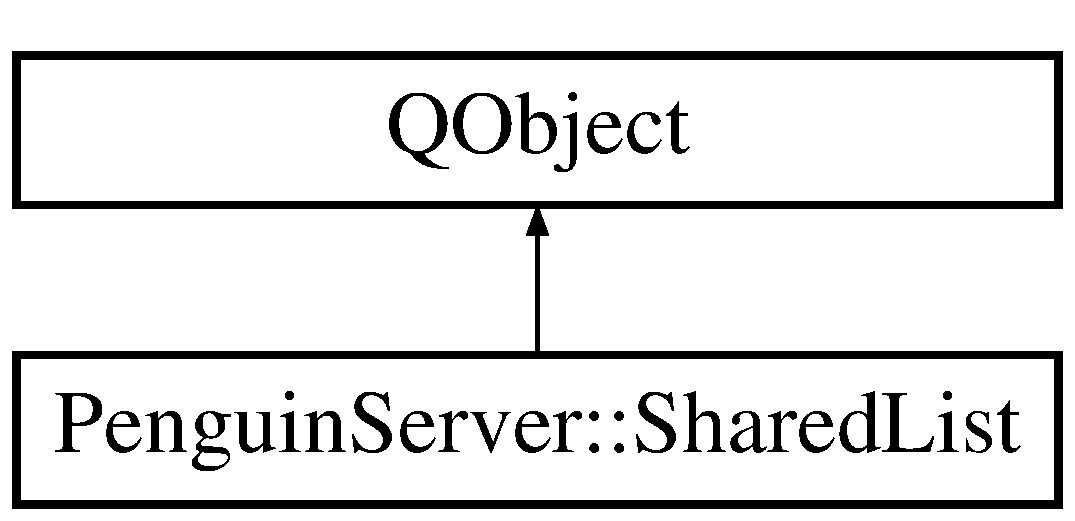
\includegraphics[height=2.000000cm]{classPenguinServer_1_1SharedList}
\end{center}
\end{figure}
\subsection*{Public Member Functions}
\begin{DoxyCompactItemize}
\item 
\hypertarget{classPenguinServer_1_1SharedList_a228585856adff620e9824e05136f1a65}{\hyperlink{classPenguinServer_1_1SharedList_a228585856adff620e9824e05136f1a65}{Shared\-List} ()}\label{classPenguinServer_1_1SharedList_a228585856adff620e9824e05136f1a65}

\begin{DoxyCompactList}\small\item\em \hyperlink{classPenguinServer_1_1SharedList}{Shared\-List}. \end{DoxyCompactList}\item 
bool \hyperlink{classPenguinServer_1_1SharedList_ab64f1d39eaaea4fcf299364a7e535270}{add\-Client} (\hyperlink{classPenguinServer_1_1ConnectedClient}{Connected\-Client} $\ast$)
\begin{DoxyCompactList}\small\item\em add\-Client \end{DoxyCompactList}\item 
bool \hyperlink{classPenguinServer_1_1SharedList_a5a6108894a1998d434ac9c9b4ec111b7}{remove\-Client} (const Q\-String \&)
\begin{DoxyCompactList}\small\item\em remove\-Client \end{DoxyCompactList}\item 
\hypertarget{classPenguinServer_1_1SharedList_a3f1af93454267de766e6d1495ca2d81e}{void \hyperlink{classPenguinServer_1_1SharedList_a3f1af93454267de766e6d1495ca2d81e}{call\-All\-Clients} ()}\label{classPenguinServer_1_1SharedList_a3f1af93454267de766e6d1495ca2d81e}

\begin{DoxyCompactList}\small\item\em call\-All\-Clients \end{DoxyCompactList}\item 
void \hyperlink{classPenguinServer_1_1SharedList_ab24885a029de18a5cd76507f4a7fb0f5}{call\-Client} (const Q\-String \&dest\-Name, const Q\-String \&src\-Name, qint16 type)
\begin{DoxyCompactList}\small\item\em call\-Client calls a client named dest\-Name witch message type tyep \end{DoxyCompactList}\end{DoxyCompactItemize}


\subsection{Detailed Description}
The \hyperlink{classPenguinServer_1_1SharedList}{Shared\-List} class. 

\subsection{Member Function Documentation}
\hypertarget{classPenguinServer_1_1SharedList_ab64f1d39eaaea4fcf299364a7e535270}{\index{Penguin\-Server\-::\-Shared\-List@{Penguin\-Server\-::\-Shared\-List}!add\-Client@{add\-Client}}
\index{add\-Client@{add\-Client}!PenguinServer::SharedList@{Penguin\-Server\-::\-Shared\-List}}
\subsubsection[{add\-Client}]{\setlength{\rightskip}{0pt plus 5cm}bool Penguin\-Server\-::\-Shared\-List\-::add\-Client (
\begin{DoxyParamCaption}
\item[{{\bf Connected\-Client} $\ast$}]{cli}
\end{DoxyParamCaption}
)}}\label{classPenguinServer_1_1SharedList_ab64f1d39eaaea4fcf299364a7e535270}


add\-Client 

\begin{DoxyReturn}{Returns}

\end{DoxyReturn}
\hypertarget{classPenguinServer_1_1SharedList_ab24885a029de18a5cd76507f4a7fb0f5}{\index{Penguin\-Server\-::\-Shared\-List@{Penguin\-Server\-::\-Shared\-List}!call\-Client@{call\-Client}}
\index{call\-Client@{call\-Client}!PenguinServer::SharedList@{Penguin\-Server\-::\-Shared\-List}}
\subsubsection[{call\-Client}]{\setlength{\rightskip}{0pt plus 5cm}void Penguin\-Server\-::\-Shared\-List\-::call\-Client (
\begin{DoxyParamCaption}
\item[{const Q\-String \&}]{dest\-Name, }
\item[{const Q\-String \&}]{src\-Name, }
\item[{qint16}]{type}
\end{DoxyParamCaption}
)}}\label{classPenguinServer_1_1SharedList_ab24885a029de18a5cd76507f4a7fb0f5}


call\-Client calls a client named dest\-Name witch message type tyep 


\begin{DoxyParams}{Parameters}
{\em dest\-Name} & whom \\
\hline
{\em src\-Name} & who \\
\hline
{\em type} & of message \\
\hline
\end{DoxyParams}
\hypertarget{classPenguinServer_1_1SharedList_a5a6108894a1998d434ac9c9b4ec111b7}{\index{Penguin\-Server\-::\-Shared\-List@{Penguin\-Server\-::\-Shared\-List}!remove\-Client@{remove\-Client}}
\index{remove\-Client@{remove\-Client}!PenguinServer::SharedList@{Penguin\-Server\-::\-Shared\-List}}
\subsubsection[{remove\-Client}]{\setlength{\rightskip}{0pt plus 5cm}bool Penguin\-Server\-::\-Shared\-List\-::remove\-Client (
\begin{DoxyParamCaption}
\item[{const Q\-String \&}]{t\-R}
\end{DoxyParamCaption}
)}}\label{classPenguinServer_1_1SharedList_a5a6108894a1998d434ac9c9b4ec111b7}


remove\-Client 

\begin{DoxyReturn}{Returns}

\end{DoxyReturn}


The documentation for this class was generated from the following files\-:\begin{DoxyCompactItemize}
\item 
sharedlist.\-h\item 
sharedlist.\-cpp\end{DoxyCompactItemize}

%--- End generated contents ---

% Index
\newpage
\phantomsection
\addcontentsline{toc}{part}{Index}
\printindex

\end{document}
